\documentclass[12pt, psamsfonts]{amsart}

%-------Packages---------
\usepackage{amssymb,amsfonts}
\usepackage{fullpage}
\usepackage{todonotes}
\usepackage{physics}
\usepackage[all,arc]{xy}
\usepackage{enumerate}
\usepackage{mathrsfs}
\usepackage{theoremref}
\usepackage{graphicx}
\usepackage[bookmarks]{hyperref}

%--------Theorem Environments--------
%theoremstyle{plain} --- default
\newtheorem{thm}{Theorem}[section]
\newtheorem{cor}[thm]{Corollary}
\newtheorem{prop}[thm]{Proposition}
\newtheorem{lem}[thm]{Lemma}
\newtheorem{conj}[thm]{Conjecture}
\newtheorem{quest}[thm]{Question}

\theoremstyle{definition}
\newtheorem{defn}[thm]{Definition}
\newtheorem{defns}[thm]{Definitions}
\newtheorem{con}[thm]{Construction}
\newtheorem{exmp}[thm]{Example}
\newtheorem{exmps}[thm]{Examples}
\newtheorem{notn}[thm]{Notation}
\newtheorem{notns}[thm]{Notations}
\newtheorem{addm}[thm]{Addendum}
\newtheorem*{exer}{Exercise}

\theoremstyle{remark}
\newtheorem{rem}[thm]{Remark}
\newtheorem{rems}[thm]{Remarks}
\newtheorem{warn}[thm]{Warning}
\newtheorem{sch}[thm]{Scholium}

\DeclareMathOperator{\Hom}{Hom}
\DeclareMathOperator{\Id}{Id}

\makeatletter
\let\c@equation\c@thm
\makeatother
\numberwithin{equation}{section}

\bibliographystyle{plain}

\begin{document}

\title{Math 611 (Due 10/2)}
\author{Hidenori Shinohara}
\maketitle

\begin{exer}{(Problem 10, Chapter 1.3)}
  Find all the connected 2-sheeted and 3-sheeted covering spaces of $S^1 \vee S^1$, up to isomorphisms of covering spaces without base points.
\end{exer}

\begin{proof}
  \todo[inline]{
    For the first part, I ended up with the two graphs in Figure \ref{fig:problem10_idea}.
    \begin{itemize}
      \item
        There have to be exactly two points in a covering space with 4 edges.
      \item
        Every other point has a neighborhood such that the point has only two edges.
      \item
        A covering space has to be path connected.
    \end{itemize}
    Based on these three things, it's not hard to get to the following two possibilities.
    However, I'm not sure if this is rigorous enough.
    Also, I don't know how this can be applied to the case of 3.
    There are many ways to connect vertices and it doesn't seem doable, which suggests that there might be better ways to solve this.
  }
 \begin{figure}
   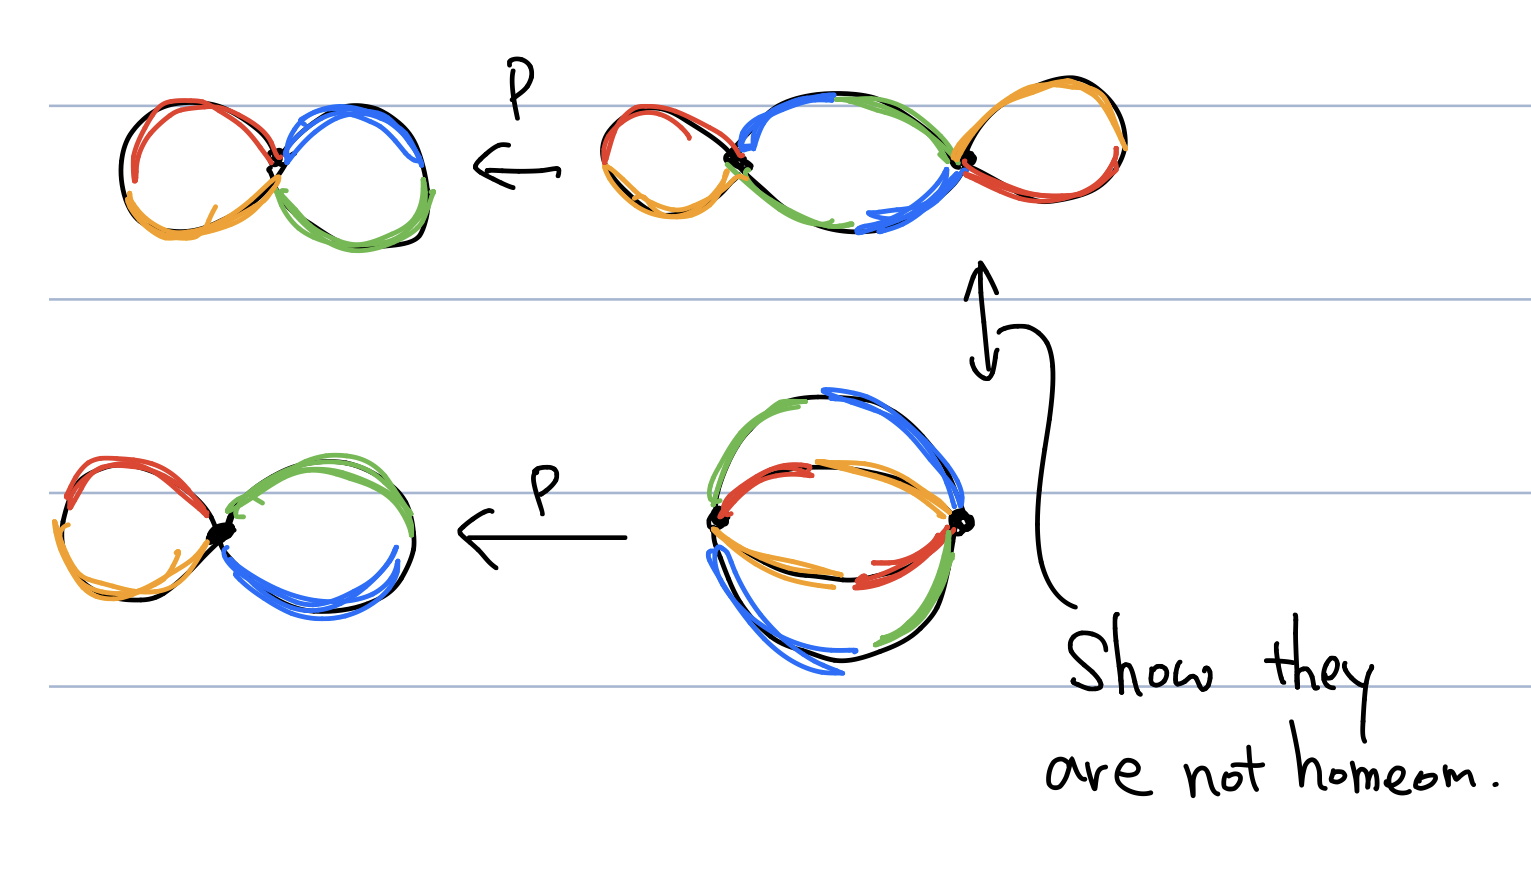
\includegraphics[width=.5\linewidth]{problem10_idea.jpeg}
   \caption{Problem 10 Idea}
   \label{fig:problem10_idea}
 \end{figure}
\end{proof}

\begin{exer}{(Problem 11, Chapter 1.3)}
  Construct finite graphs $X_1$ and $X_2$ having a common finite-sheeted covering space $\tilde{X}_1 = \tilde{X}_2$, but such that there is no space having both $X_1$ and $X_2$ as covering spaces.
\end{exer}

\begin{proof}
  \todo[inline]{
    Since they are finite graphs, we can analyze the degree of each vertex.
    The degree of each vertex is preserved when lifted, so that's something I'm trying to make use of. 
    So, something like Figure \ref{fig:problem11_idea} is what I'm trying to do.
    The idea is that $X_1, X_2$ would have 2 and 3 vertices with degree 4, so $X$ must have exactly one vertex with degree 4.
    However, in this case, $S \vee S$ has both $X_1$ and $X_2$ as covering spaces.
    I've also tried graphs with vertices of different degrees like 3.
    I think this is the right approach. I just need some more time.
  }
 \begin{figure}
   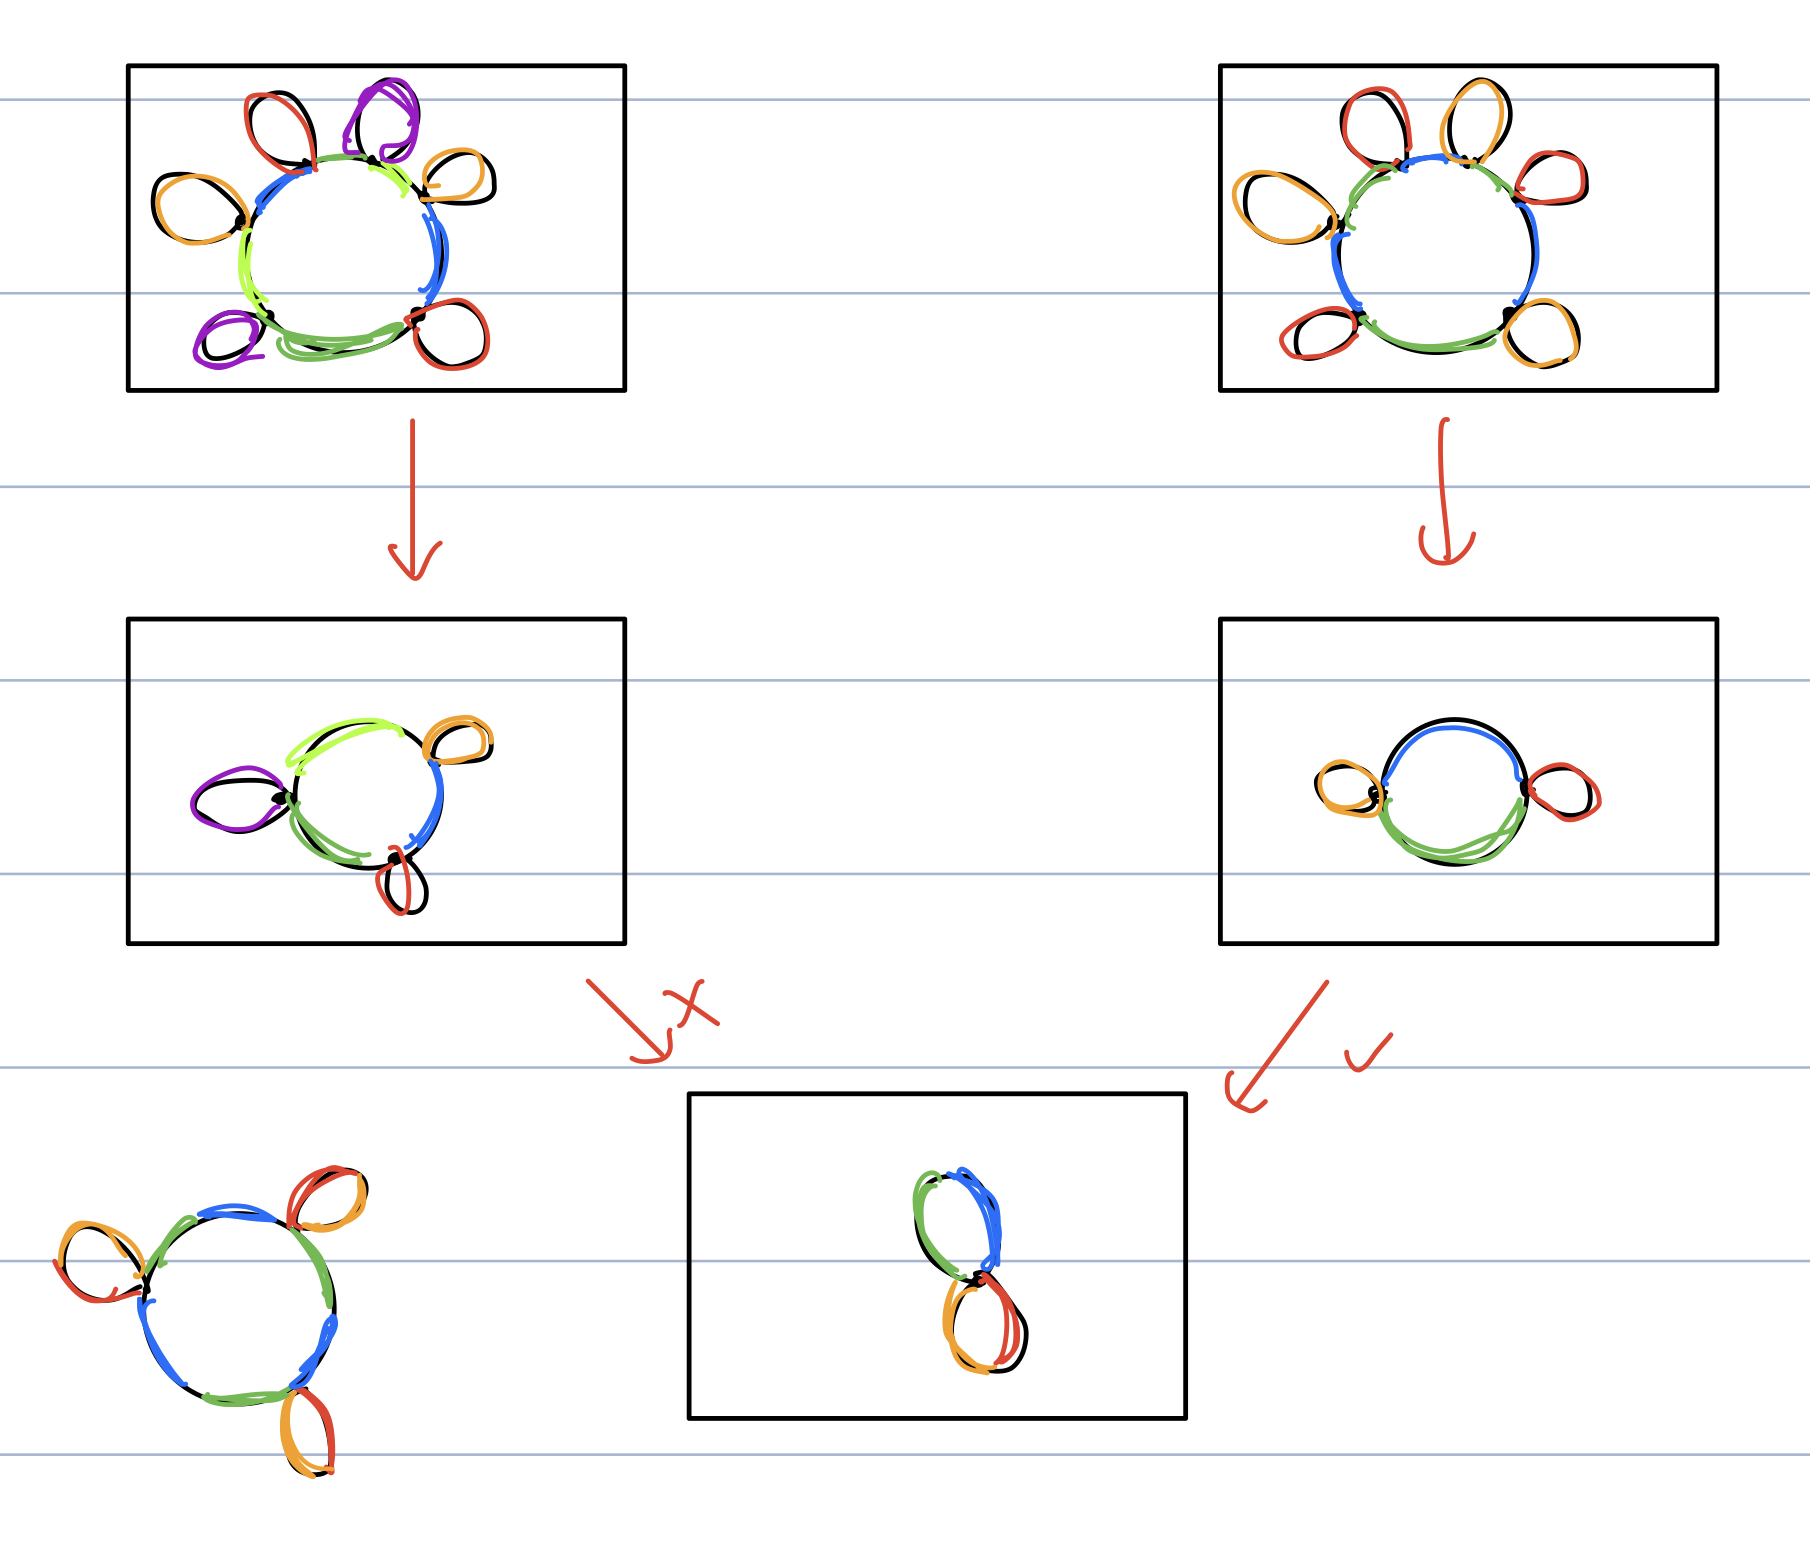
\includegraphics[width=.5\linewidth]{problem11_idea.jpeg}
   \caption{Problem 11 Idea}
   \label{fig:problem11_idea}
 \end{figure}
\end{proof}

\begin{exer}{(Problem 14, Chapter 1.3)}
  Find all the connected covering spaces of $\mathbb{R}P^2 \vee \mathbb{R}P^2$.
\end{exer}

\begin{proof}
  \todo[inline]{
    A sphere is a 2-sheeted covering space of $\mathbb{R}P^2$.
    Moreover, it is simply connected, so I guess that means it's a universal covering.
    Since the universal covering is 2 sheeted, I feel that it limits the possibilities.
    I wonder if Figure \ref{fig:problem14_idea} is indeed a covering space.
    If it is, this might be the only nontrivial one?
    I'm not certain.
  }
  \begin{figure}
    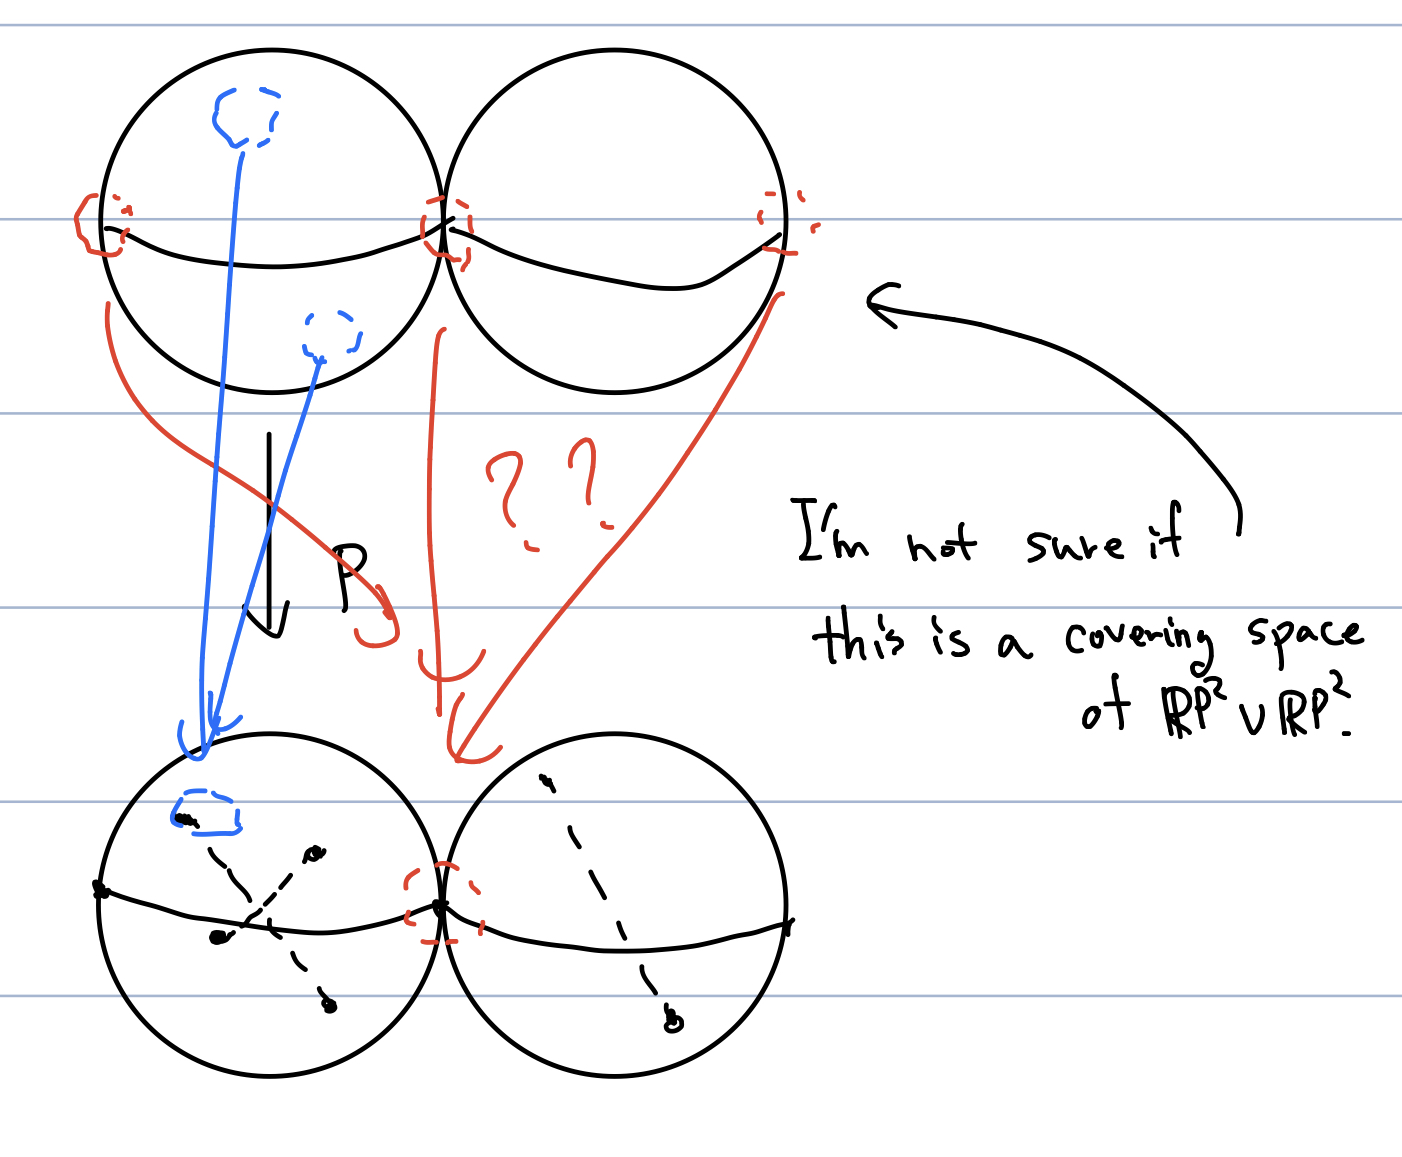
\includegraphics[width=.5\linewidth]{problem14_idea.jpeg}
    \caption{Problem 14 Idea}
    \label{fig:problem14_idea}
  \end{figure}
\end{proof}

\end{document}


